\documentclass[twoside,11pt]{article}

% Any additional packages needed should be included after jmlr2e.
% Note that jmlr2e.sty includes epsfig, amssymb, natbib and graphicx,
% and defines many common macros, such as 'proof' and 'example'.
%
% It also sets the bibliographystyle to plainnat; for more information on
% natbib citation styles, see the natbib documentation, a copy of which
% is archived at http://www.jmlr.org/format/natbib.pdf

\usepackage{jmlr2e}
\usepackage{minted}
\usepackage{graphicx}
\usepackage{caption}
\usepackage{subcaption}
\usepackage{stmaryrd}
\usepackage[colorinlistoftodos]{todonotes}

% Definitions of handy macros can go here

\newcommand{\dataset}{{\cal D}}
\newcommand{\fracpartial}[2]{\frac{\partial #1}{\partial  #2}}

% Heading arguments are {volume}{year}{pages}{submitted}{published}{author-full-names}

\jmlrheading{}{}{}{}{}{William de Vazelhes and CJ Carey and Yuan Tang and Nathalie Vauquier and Aur\'elien Bellet}

% Short headings should be running head and authors last names

\ShortHeadings{Metric-learn: Metric Learning in Python}{de Vazelhes, Carey, Tang, Vauquier and Bellet}
\firstpageno{1}

\begin{document}

\title{Metric-learn: Metric Learning in Python}

\author{\name William de Vazelhes \email william.de-vazelhes@inria.fr \\
       \addr INRIA, France
       \AND
       \name CJ Carey \email perimosocordiae@gmail.com \\
       \addr \todo[inline]{TODO}
       \AND
       \name Yuan Tang \email terrytangyuan@gmail.com \\
       \addr \todo[inline]{TODO}
       \AND
       \name Nathalie Vauquier \email nathalie.vauquier@inria.fr \\
       \addr INRIA, France
       \AND
       \name Aur\'elien Bellet \email aurelien.bellet@inria.fr \\
       \addr INRIA, France
       }

\editor{}

\maketitle

\begin{abstract}%   <- trailing '%' for backward compatibility of .sty file
\texttt{metric-learn} is an open source Python package for metric-learning, based on \texttt{numpy}, \texttt{scipy}, and \texttt{scikit-learn}. It allows to learn a metric between data points that satisfy desired properties. \texttt{metric-learn} stands out from other packages by providing a unified interface for metric learning with several modes of supervision (full supervision or pairs and quadruplets supervision), all being compatible with \texttt{scikit-learn} and allowing to do cross-validation, model selection, and pipelining. The package is released under the MIT licence, and the current version (v0.5.0) is downloadable from PyPi. The source code is available online at \url{http://github.com/metric-learn/metric-learn}, as well as the documentation at \url{http://metric-learn.github.io/metric-learn/}.
\end{abstract}




\begin{keywords}
  Machine Learning, Python, Metric Learning, Scikit-learn
\end{keywords}

\section{Introduction}

Many approaches in machine learning require a measure of distance between data
points. Traditionally, practitioners would choose a standard distance metric
(Euclidean, City-Block, Cosine, etc.) using a priori knowledge of the
domain. However, it is often difficult to design metrics that are well-suited
to the particular data and task of interest.
% \todo[inline]{probably need to add a sentence explaining what is meant by weak supervision}
Distance metric learning  (or simply, metric learning) (\cite{Bellet13}, \cite{Kulis13}, \cite{Surez18}) aims at
automatically constructing task-specific distance metrics from data, in a machine learning manner. It can deal with various types of supervision: either full supervision, where we know label(s) for each sample, or weaker supervision, where we only have some information about the similarities between samples. The learned distance metric can
then be used to perform various tasks, for instance to retrieve the elements (images, documents) of a database that are semantically closer to a query element. It can also be plugged into other machine learning algorithms: popular use-cases include improving the accuracy of nearest neighbors learning models (for classification, regression, anomaly detection...) or biasing the clusters found by clustering algorithms like K-Means towards the intended semantics. Finally, metric learning can be used to perform dimensionality reduction.
These use-cases highlight the importance of integrating metric learning into the rest of the machine learning pipeline and tools.
% \todo[inline]{quick presentation of the package: implements several algorithms, with sklearn-compatible API for model selection, model evaluation, pipelining with other estimators. makes metric-learn stands out from other packages (maybe mention a few of them), in particular in the case of weakly supervised algorithms}
\texttt{metric-learn} is a package for metric learning in Python, which provides many common metric-learning algorithms unified through a common interface. It allows to do metric-learning with different level of supervision.
% (not only class supervision, unlike most packages are focused on, including another package for metric learning in Python, \texttt{PyDML})
% , which is one interesting feature allowed by the metric learning paradigm. 
Its API is compatible with scikit-learn, the leading library for machine learning in Python, allowing for model selection, evaluation, and pipelining, which makes \texttt{metric-learn} stand out from other packages, like \texttt{PyDML} \footnote{\url{https://github.com/jlsuarezdiaz/pyDML}}, which mostly focuses on supervised metric learning algorithms.
% Acknowledgements should go at the end, before appendices and references
The rest of this paper is organized as follows. We first present an overview of the package, followed by a more detailed description of the available algorithms. We then give more details about the API and the software architecture, in particular the compatibility with \texttt{scikit-learn}, and conclude with a discussion of future developments.


\section{Overview of the Package}

\texttt{metric-learn} only relies on core libraries from the SciPy ecosystem: \texttt{numpy}, \texttt{scipy}, and \texttt{scikit-learn}.\footnote{An optional dependency with \texttt{skggm} (\cite{skggm}) can be installed in order to use a more stable solver when using the LSML algorithm from the package.}
The current release (v.0.5.0) can be installed from the Python Package Index (PyPI), for python 2.7 and 3.5 or later. The source code is available on GitHub at \url{http://github.com/metric-learn/metric-learn}. The development is collaborative and open to all contributors through the usual GitHub framework (issues and pull requests). The code is free of use, provided under the MIT licence. The interest of the package from the community is clear, since the project has been starred more than 730 times and forked more than 170 times at the time of writing.
A detailed documentation, including installation guidelines, the description of the algorithms and the API, as well as example of use done with \texttt{sphinx-gallery}, is available at \url{https://metric-learn.github.io/metric-learn/}. The quality of the code is ensured by an intensive test coverage of 96\%. Every new contribution to the code is automatically checked by a continuous integration platform that ensures a minimal test coverage of the added code, and an minimal variation in test coverage of the overall code, which allows easy contribution for incoming developers, which can have their code automatically checked.

\section{Available algorithms}
% \todo[inline]{comparison with other packages ? }
% Metric learning problems fall into two main categories depending on the type
% of supervision available about the training data:

% \begin{itemize}
%     \item 
% - Supervised learning: the algorithm has access to
%   a set of data points, each of them belonging to a class (label) as in a
%   standard classification problem.
%   Broadly speaking, the goal in this setting is to learn a distance metric
%   that puts points with the same label close together while pushing away
%   points with different labels.
% - Weakly supervised learning: the
%   algorithm has access to a set of data points with supervision only
%   at the tuple level (typically pairs, triplets, or quadruplets of
%   data points). A classic example of such weaker supervision is a set of
%   positive and negative pairs: in this case, the goal is to learn a distance
%   metric that puts positive pairs close together and negative pairs far away.


% \end{itemize}


\paragraph{General setting} Metric learning problems are generally formulated as an optimization problem where one seeks to find, on the training data $(x_0, ..., x_n)$, the parameters $\theta$ of a distance function $D_\theta(x_i, x_j)$ that optimize some desired objective function $\mathcal{L}_\theta(x_0, ..., x_n) = f(D_\theta(x_0, x_0), ..., D_\theta(x_0, x_n), ..., D_\theta(x_n, x_0), ..., D_\theta(x_n, x_n))$, hoping that this metric will generalize the desired propertie(s) on new incoming test data.

\subparagraph{Mahalanobis metric learning}

In the metric-learn package, all algorithms currently implemented learn so-called Mahalanobis distances. Given a real-valued parameter matrix $L$ of shape \texttt{(num\_dims, n\_features)} where \texttt{n\_features} is the
number of features describing the data, the Mahalanobis distance associated with
$L$ is defined as follows:

$D(x, x') = \sqrt{(Lx-Lx')^\top(Lx-Lx')}$

In other words, a Mahalanobis distance is a Euclidean distance after a
linear transformation of the feature space defined by $L$ (taking
$L$ to be the identity matrix recovers the standard Euclidean distance).
Mahalanobis distance metric learning can thus be seen as learning a new
embedding space of dimension \texttt{num\_dims}. Note that when \texttt{num\_dims} is
smaller than \texttt{n\_features}, this achieves dimensionality reduction.

% Strictly speaking, Mahalanobis distances are "pseudo-metrics": they satisfy
% three of the properties of a metric (non-negativity, symmetry, triangle inequality) but not
% necessarily the identity of indiscernibles.

% Mahalanobis distances can also be parameterized by a positive semi-definite 
% (PSD) matrix $M$:

% $ D(x, x') = \sqrt{(x-x')^\top M(x-x')}$

% Using the fact that a PSD matrix :math:`M` can always be decomposed as
% $M=L^\top L$ for some  :math:`L`, one can show that both
% parameterizations are equivalent. In practice, an algorithm may thus solve
% the metric learning problem with respect to either :math:`M` or :math:`L`.

\paragraph{Supervised Learners}
The first possibility to learn this metric is from class supervision. We can learn a metric that brings closer together points from the same class and spreads further away points from a different class. For instance, in figure \ref{fig:full}, the class is the identity of a person of an image, and we want to put closer together images from the same person.Currently, \texttt{metric-learn} contains the following algorithms for full supervision: Neighborhood Components Analysis (NCA) (\cite{Goldberger04}), Large Margin Nearest Neighbors (LMNN) (\cite{Weinberger09}), Relative Components Analysis (RCA) (\cite{Shental02}), Local Fisher Discriminant Analysis (LFDA) (\cite{Sugiyama07}) and Metric Learning for Kernel Regression (MLKR) (\cite{Weinberger07}) (which uses a continuous label like in regressions, instead of a class label).

% \todo[inline]{ces figures ne sont pas très vendeuses. je propose de faire une figure conceptuelle en prenant l'exemple des faces expliquant la différence entre le supervisé, les paires et les quadruplets. on peut s'inspirer de \url{http://cedric.cnam.fr/~thomen/papers/Law_ICCV_2013_QWise.pdf}}

% \begin{figure}[H]
% \centering
% \begin{subfigure}{.5\textwidth}
%   \centering
%   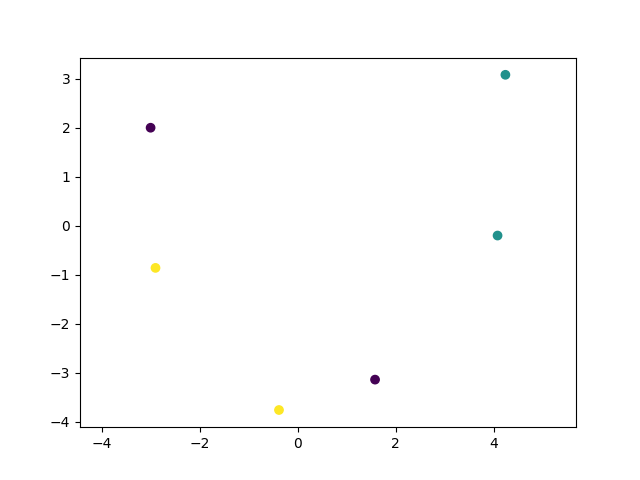
\includegraphics[width=.8\linewidth]{supervised_without_metric.png}
%   \caption{Original points, before metric learning}
%   \label{fig:sub1}
% \end{subfigure}%
% \begin{subfigure}{.5\textwidth}
%   \centering
%   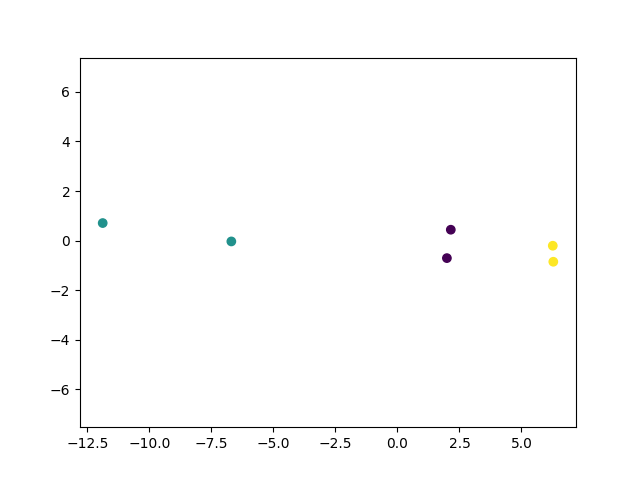
\includegraphics[width=.8\linewidth]{supervised_with_metric.png}
%   \caption{points after metric learning (ITML)}
%   \label{fig:sub2}
% \end{subfigure}
% \caption{Metric learning with pairwise constraints}
% \label{fig:test}
% \end{figure}


% \paragraph{Weakly Supervised Metric Learning algorithms}
% Weakly Supervised algorithms use less information than the previous algorithms: they only take tuple of points and possibly a corresponding label. See below for more concrete examples of algorithms learning on tuples.
\subparagraph{Pairs Learners} 
Another way is to have pair of points as inputs, and a corresponding label indicating whether the two points are similar or not. We can then learn a metric that brings points from a similar pair closer together, and points from a dissimilar pair further away from each other. For instance, we could want to put closer together in the embedding space images from the same person (i.e. similar), and further away images from a different person (i.e. dissimilar) (see figure \ref{fig:pairs}). Currently, \texttt{metric-learn} contains the following algorithms for pairs supervision: Mahalanobis Metric for Clustering (MMC) (\cite{Xiang08}), Sparse High-Dimensional Metric Learning (SDML) (\cite{Qi09}), Information Theoretic Metric Learning (ITML) (\cite{Davis07}).
    

    

% \begin{figure}[H]
% \centering
% \begin{subfigure}{.5\textwidth}
%   \centering
%   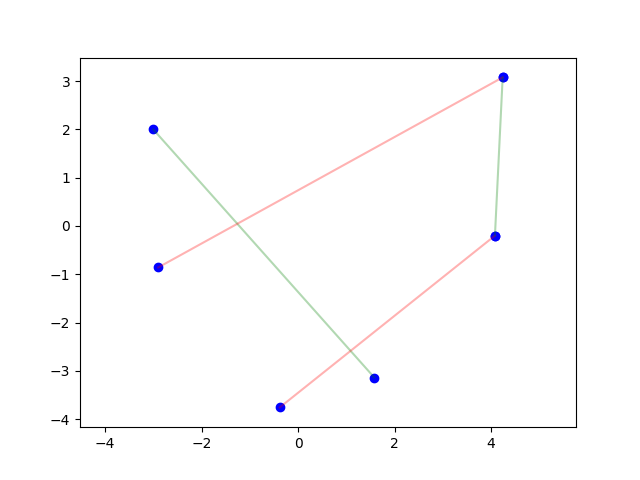
\includegraphics[width=.8\linewidth]{pairs_without_metric.png}
%   \caption{Original points, before metric learning}
%   \label{fig:sub1}
% \end{subfigure}%
% \begin{subfigure}{.5\textwidth}
%   \centering
%   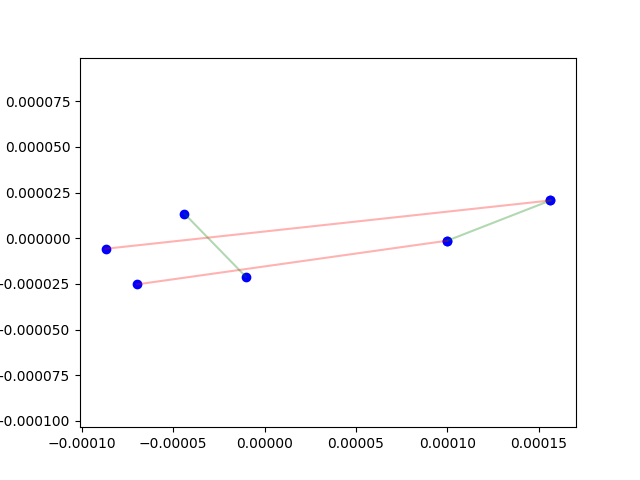
\includegraphics[width=.8\linewidth]{pairs_with_metric.png}
%   \caption{points after metric learning (ITML)}
%   \label{fig:sub2}
% \end{subfigure}
% \caption{Metric learning with pairwise constraints}
% \label{fig:test}
% \end{figure}
    
\subparagraph{Quadruplets Learners}
The last possibility to learn a metric in \texttt{metric-learn} currently is to take as input quadruplets of points. We will learn a metric that brings the two first points of each quadruplet closer than the two last points are. This can be used for instance to learn a metric space in which closer points have closer values of a given attributes. In figure \ref{fig:quadruplets} for instance, we want to learn a metric that puts closer together people from approximately the same age. Currently the only algorithm in \texttt{metric-learn} for learning on quadruplets is Metric Learning from Relative Comparisons by Minimizing Squared Residual (LSML) (\cite{Liu12}).





\begin{figure}[H]
  \centering
  \begin{subfigure}[t]{0.3\textwidth}
     \centering 
     \begin{tabular}{c|c}
     \texttt{X} & \texttt{y} \\ \hline \\
   
\includegraphics[scale=0.15]{Tom_Cruise_0010.jpg} & 'Tom' \\
   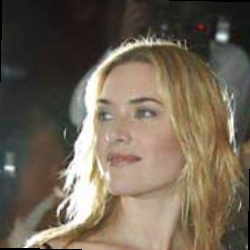
\includegraphics[scale=0.15]{Kate_Winslet_0001.jpg} & 'Kate' \\
\end{tabular}
     \caption{}
     \label{fig:full}
     \end{subfigure}
  \hspace{5pt}
  \begin{subfigure}[t]{0.3\textwidth}
     \centering
     \begin{tabular}{c|c}
     \texttt{pairs} & \texttt{y\_pairs} \\  \hline \\
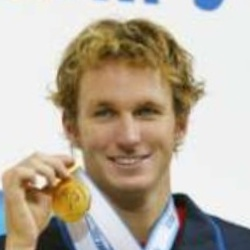
\includegraphics[scale=0.15]{Aaron_Peirsol_0001.jpg} 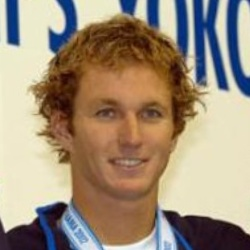
\includegraphics[scale=0.15]{Aaron_Peirsol_0002.jpg} & 1\\  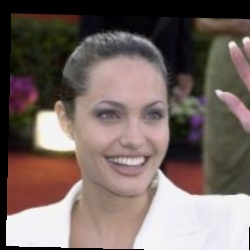
\includegraphics[scale=0.15]{Angelina_Jolie_0001.jpg}   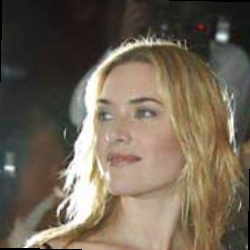
\includegraphics[scale=0.15]{Kate_Winslet_0001.jpg} & -1 \\
\end{tabular}
     \caption{}
     \label{fig:pairs}
  \end{subfigure}
  \hspace{5pt}
  \begin{subfigure}[t]{0.3\textwidth}
     \centering 
     
          \begin{tabular}{c}
     \texttt{quadruplets} \\ \hline \\
     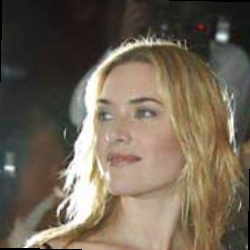
\includegraphics[scale=0.15]{Kate_Winslet_0001.jpg} 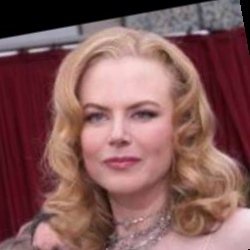
\includegraphics[scale=0.15]{Nicole_Kidman_0001.jpg} 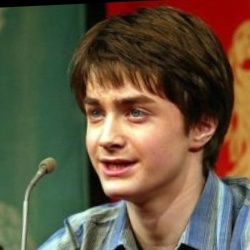
\includegraphics[scale=0.15]{Daniel_Radcliffe_0001.jpg} 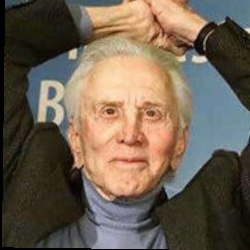
\includegraphics[scale=0.15]{Kirk_Douglas_0001.jpg} \\
          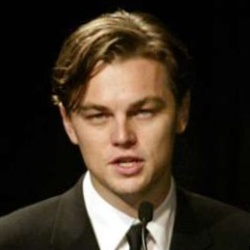
\includegraphics[scale=0.15]{Leonardo_DiCaprio_0001.jpg} 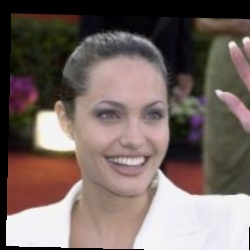
\includegraphics[scale=0.15]{Angelina_Jolie_0001.jpg} 
\includegraphics[scale=0.15]{Daryl_Sabara_0001.jpg} 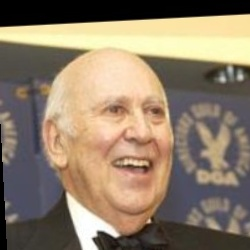
\includegraphics[scale=0.15]{Carl_Reiner_0002.jpg} \\
\end{tabular}
    
     
     \caption{}
     \label{fig:quadruplets}
  \end{subfigure}
  \caption{Different types of supervision. \textbf{\ref{fig:full} Full supervision:} we want samples from the same label to be closer than samples from different labels. \textbf{\ref{fig:pairs} Pairs supervision:} we want similar samples (1) (the same person) to be closer than dissimilar samples (-1) (different persons). \textbf{\ref{fig:quadruplets} Quadruplets supervision:} no labels. We want the two leftmost samples (not much age difference) to be closer than the two rightmost samples (bigger age difference).}
  \label{fig:contour}
\end{figure}

\section{Software Architecture and API}

\texttt{metric-learn}'s goal is to provide a unified interface to all metric-learning algorithms, including the ones that have an input format that differs from classical machine learning ones, and allow to combine them with scikit-learn objects. As such, all metric-learners from \texttt{metric-learn} inherit from an abstract \texttt{BaseMetricLearner} object.
% \todo[inline]{Should I talk about the classes etc ? Not useful since they are not visible by the user right ?}
% \todo[inline]{I think it can be nice, this is not documentation, but explaining how things are coded}

\texttt{metric-learn}'s API is designed to be fully compatible with \texttt{scikit-learn} API (\cite{scikit-learn}). 

\paragraph{Mahalanobis metric learning}

Since they learn a Mahalanobis matrix, all algorithm also inherit from the \texttt{MahalanobisMixin} interface. This latter can return the mahalanobis matrix with the method \texttt{get\_mahalanobis\_matrix}. Like scikit-learn's algorithms, it can also return a \texttt{components\_} attributes that is the transformation matrix \texttt{L}. Since all these metric learner learn this implicit transformation $L$, they can project the input in the new space using \texttt{transform}. A distance function can also be extracted from them using \texttt{get\_metric}, that can further be used in any scikit-learn estimator like \texttt{KMeansClustering}. They can also return the distance between a dataset of pairs (in the 3D array format (see below), using \texttt{score\_pairs}.



\paragraph{Supervised metric learners}


Supervised metric learners inherit from scikit-learn base class \texttt{TransformerMixin}, just like \texttt{scikit-learn}'s \texttt{LinearDiscriminantAnalysis} for instance, and they behave as such.
% (they pass all scikit-learn's "estimators checks"). 
%  They can easily be pipelined with nearest neighbors estimators to improve their performance: \texttt{better\_knn = sklearn.pipeline.make\_pipeline(NCA(), KNeighborsClassifier())} (TODO: sth to explain NCA is in metric-learn)


\paragraph{Weakly Supervised metric learners} 
% Algorithms that learn on pairs or quadruplets take as input 3D array of shape \texttt{(n\_samples, t, n\_features)} (where...). In other words, sampling one element along the first dimension returns one tuple (e.g. a pair), that is a matrix of t lines corresponding to the t elements in the tuple.
% This format is what allows all these API choices, since slicing along the 1st dimension
% While a classical input array \texttt{X} in \texttt{scikit-learn} has shape \texttt{(n\_samples, n\_features)}, an array of tuples has shape \texttt{(n\_tuples, t, n\_features)}, where \texttt{t} is the number of elements in a tuple (e.g. 2 for pairs).
% Note that \texttt{scikit-learn} accepts arrays in a broad sense, in what they call "array-like" objects. \texttt{metric-learn} too accepts "tuple-like" objects.
Weakly supervised learning algorithms are similar to \texttt{scikit-learn} classifiers, but they \texttt{fit} on tuples that can be given as 3D arrays, instead of 2D arrays-like of points \texttt{X}. They have a \texttt{predict} method, that gives a prediction for each given tuple (e.g. for pairs it predicts whether the two points in a pair or similar or not). Tuples can be pairs or quadruplets, depending on the specific algorithm used. Below is a code example for pairs supervision:

\begin{minted}{python}
import numpy as np
from metric_learn import MMC
pairs = np.array([[[1.2, 3.2], [2.3, 5.5]], [[4.5, 2.3], [2.1, 2.3]]])
y_pairs = np.array([1, -1])
mmc = MMC()
mmc.fit(pairs, y_pairs)
\end{minted}
% mmc.predict(pairs)


This allows to use out of the box \texttt{scikit-learn}'s scoring functions, and therefore all routines for model selection, including the \texttt{GridSearchCV} object. Also note that for every weakly supervised learner, there is a \texttt{\_Supervised} version (e.g. for \texttt{MMC} there is \texttt{MMC\_Supervised}, that is a supervised version that samples pairs of similar samples from intra-class samples, and dissimilar samples from inter-class samples, and fits \texttt{MMC} on these pairs).


% \begin{minted}{python}
% from sklearn.model_selection import GridSearchCV
% model = GridSearchCV(mmc, {'init': ['random', 'identity', 'covariance']})
% model.fit(pairs, y_pairs)
% \end{minted}

\section{Conclusion and Future Work}


In conclusion, we presented a scikit-learn compatible package for metric-learning. This package is under active development and many improvements are planned to be added to the package. First, the scalability of the package could be improved by supporting stochastic solvers (like stochastic gradient descent), and/or to form pairs on the fly and do computations by batch, in order not to load every sample in memory at once. We could also take advantage of possible sparse input format to reduce computations. More algorithms could also be added to the package, like algorithms learning on triplets, algorithms that can deal with high dimensional data. We could also allow metric learn to be used when having multiple labels for each sample, and allow different kind of supervisions, like semi-supervised learning for instance. We could also improve the ease of use by adding more examples and adding toy datasets to play with quickly and see the interest of the weaker forms of supervision. About the overall quality of the software, we intend to improve the continuous integration routines, for instance by ensuring a PEP8 syntax checker is run on every pull request, a continuous integration for the documentation.

\acks

We would like to be particularly thankful to Inria for funding two years of development of the package. Also we would like to thanks \texttt{scikit-learn} developers for fruitful discussions, assistance for developing the new API, and funding for conference attending.
\todo[inline]{reformulate + other acknowledgments}

%  The quality of comparison to previous (if any) related implementations, w.r.t. run-time, memory requirements, features, to explain that significant progress has been made. 

% Manual newpage inserted to improve layout of sample file - not
% needed in general before appendices/bibliography.

\bibliography{metric-learn-jmlr}

\end{document}